\documentclass[aspectratio=169]{beamer}
\usepackage{graphicx}
\title{Using agent-based modelling to explore the effect of social networks and beliefs on active travel}
\author{Robert Greener}
\institute{London School of Hygiene and Tropical Medicine}
\date{27th October 2022}

\begin{document}
\maketitle

\begin{frame}
    \frametitle{Background}
    \begin{columns}
        \begin{column}{0.5\textwidth}
            \begin{itemize}
                \item Active travel policies frame walking \& cycling as `good', cars as `bad'!
                \item Perceptions of acceptable commute method vary by groups.
                \item Beliefs may explain this difference.
                \item Beliefs spread through social networks.
            \end{itemize}
        \end{column}
        \begin{column}{0.5\textwidth}
            \begin{figure}[H]
                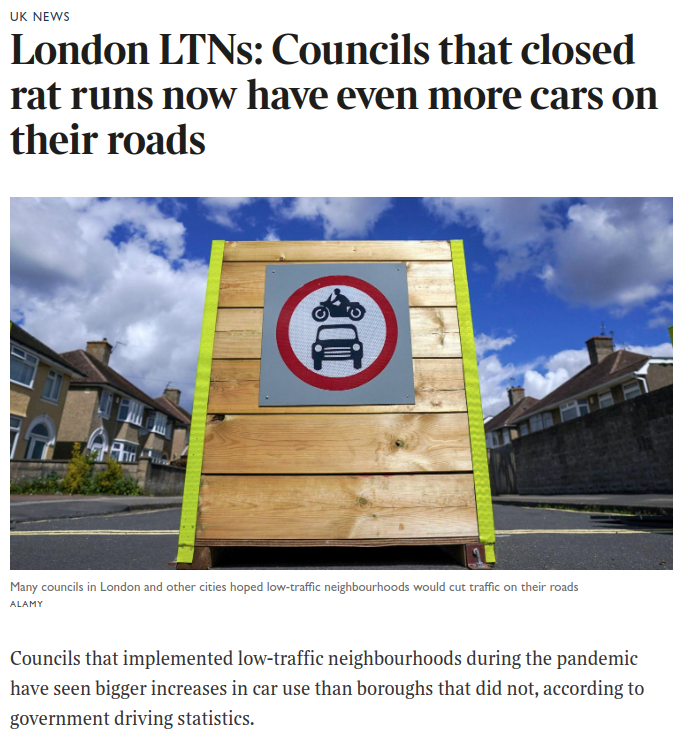
\includegraphics[width=0.7\textwidth]{figures/the-times.png}
                \caption{\emph{The Times} 24th October 2022}
            \end{figure}
        \end{column}
    \end{columns}
\end{frame}

\begin{frame}
    \frametitle{Research questions}
    \begin{enumerate}
        \item What are the beliefs and attitudes required to create a calibrated model of active travel?
              \begin{itemize}
                  \item Answered by a systematic review of the literature.
              \end{itemize}
        \item What network-based interventions may be effective in increasing active travel levels?
        \item How may non-network-based interventions cause an additional network-based effect
    \end{enumerate}
\end{frame}

\begin{frame}
    \frametitle{Next steps}
    \begin{itemize}
        \item Run this model many times. Do the results make sense?
        \item Implement some interventions. What are there results?
        \item What do the results mean for public health policy / planning policy?
        \item Is there any `low-hanging fruit'?
    \end{itemize}
\end{frame}

\begin{frame}
    \frametitle{Any questions / acknowledgements}
    \begin{itemize}
        \item Thank you for listening; any questions?
        \item Robert Greener is supported by a Medical Research Council Studentship [grant number: MR/N0136638/1].
    \end{itemize}
    \vspace*{4em}
    
\includegraphics[height=5em]{figures/LSHTM-logo-bw.jpg}
    
\includegraphics[height=5em]{figures/Medical_Research_Council_logo.svg.png}
    
\includegraphics[height=2em]{figures/philab.png}
\end{frame}
\end{document}